\newenvironment{LeftTablePage}{%
	\thispagestyle{empty}%
	% Временно уменьшаем отступы.
	\newgeometry{left=5mm, top=25mm, bottom=10mm}%
	% Содержимое слева.
	\noindent\begin{minipage}[b]{20mm}
		\rotatebox{90}{
			\begin{tabular}{| c | c | c | c | c |}
				\hline
				Инв. № подл. & Подп. и дата & Взам. инв. № & Инв. № дубл. & Подп. и дата \\
				\hline
				\docId & & & & \\
				\hline
			\end{tabular}%
		}
	\end{minipage}%
	% Основное содержимое
	\begin{samepage}%
	\begin{minipage}[b][\textheight]{\textwidth}\centering%
}{
	\end{minipage}%
	\end{samepage}
	
	% Теперь можно вернуть отступы как были
	\restoregeometry

	\clearpage
}

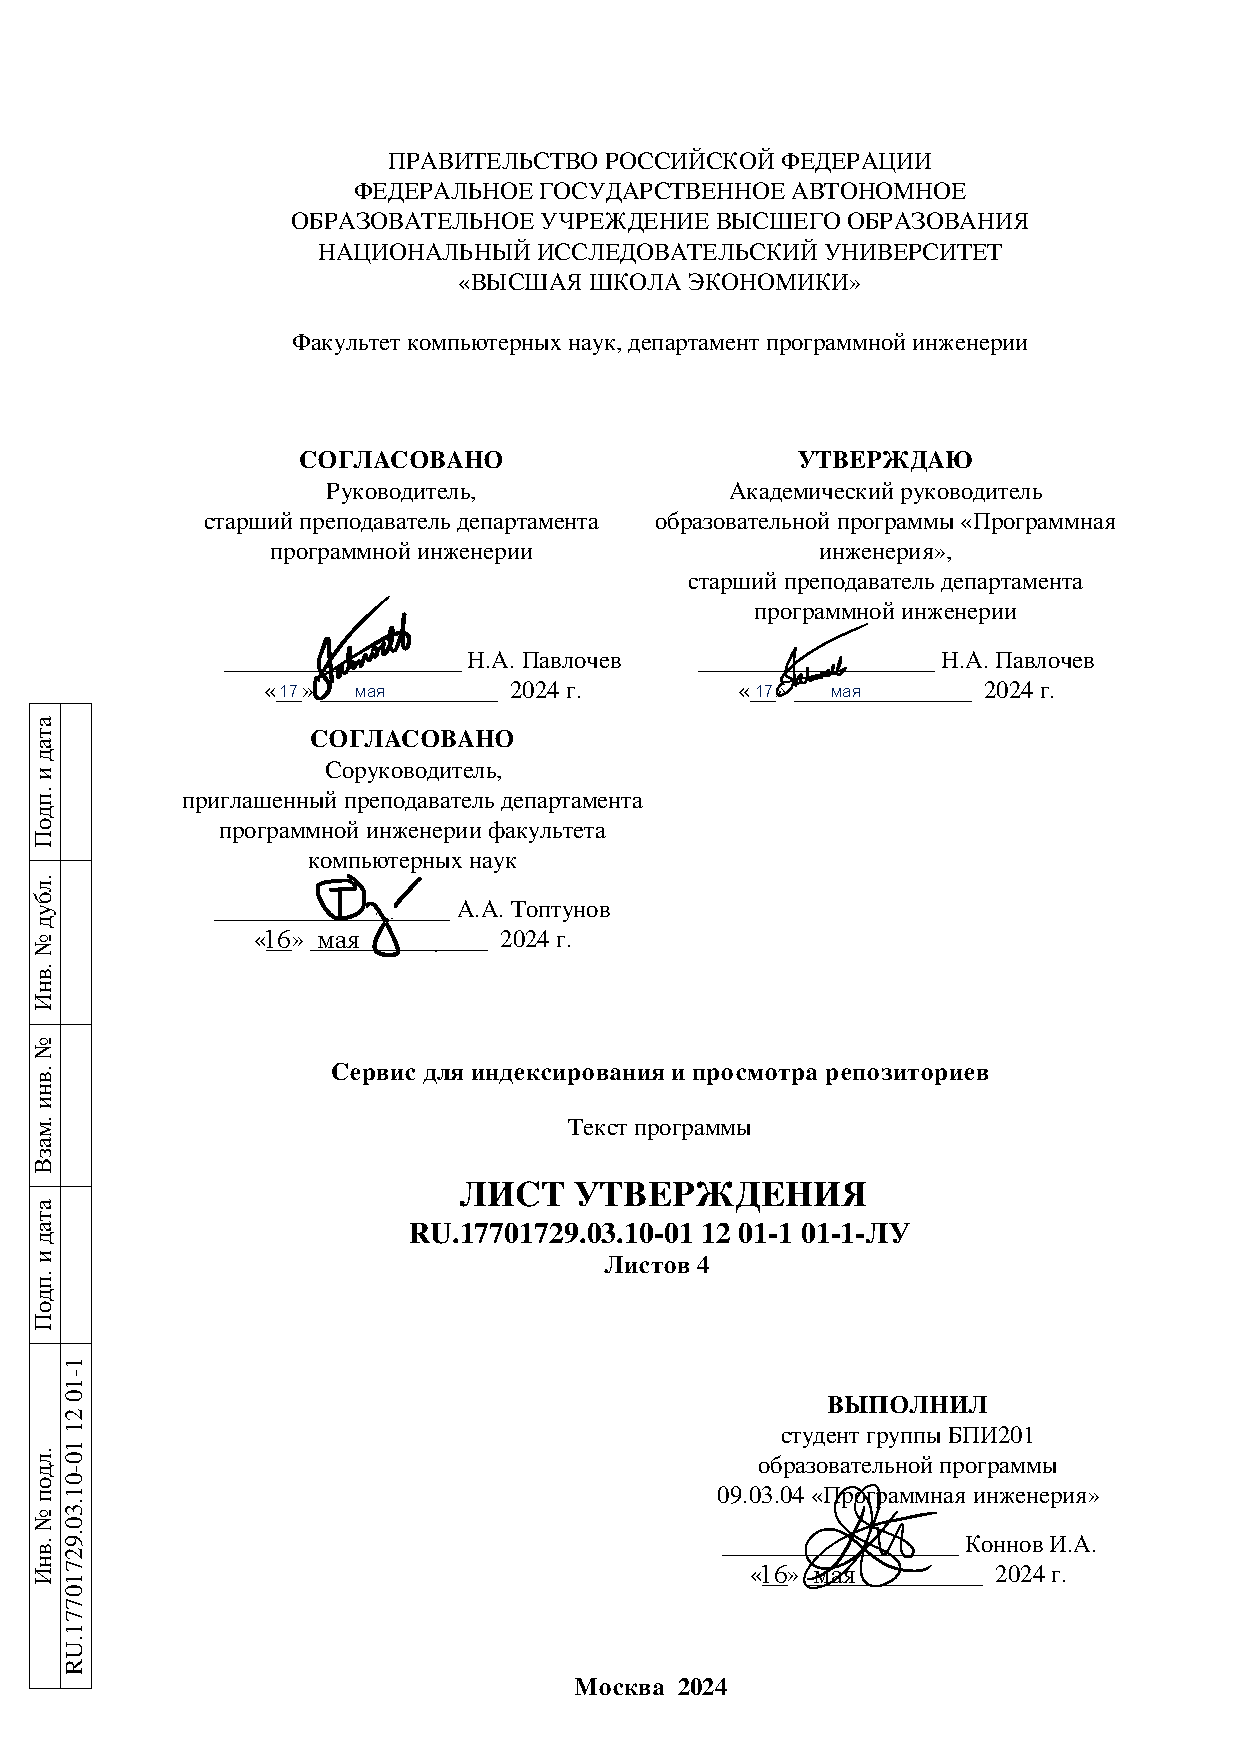
\includepdf[pages=-]{figures/signed.pdf}
% \begin{LeftTablePage}
% 	%% Лист утверждения
    ПРАВИТЕЛЬСТВО РОССИЙСКОЙ ФЕДЕРАЦИИ \\
    ФЕДЕРАЛЬНОЕ ГОСУДАРСТВЕННОЕ АВТОНОМНОЕ \\
    ОБРАЗОВАТЕЛЬНОЕ УЧРЕЖДЕНИЕ ВЫСШЕГО ОБРАЗОВАНИЯ \\
    НАЦИОНАЛЬНЫЙ ИССЛЕДОВАТЕЛЬСКИЙ УНИВЕРСИТЕТ \\
    «ВЫСШАЯ ШКОЛА ЭКОНОМИКИ» \\[1\baselineskip]
    Факультет компьютерных наук, департамент программной инженерии
\vskip 1.5cm
    % Согласовано / утверждаю
    \begin{varwidth}[t]{0.45\textwidth}\centering
    	\textbf{СОГЛАСОВАНО}
    	
    	Руководитель, \\
    	старший преподаватель департамента
        программной инженерии
    \end{varwidth}%
    \hfil%
    \begin{varwidth}[t]{0.45\textwidth}\centering
    	\textbf{УТВЕРЖДАЮ}
    	
    	Академический руководитель
        образовательной программы
        «Программная инженерия», \\
        старший преподаватель департамента
        программной инженерии
    \end{varwidth}

\bigskip

    \begin{varwidth}[t]{0.4\textwidth}\centering
    	\placename Н.А. Павлочев \\
    	\placedate
    \end{varwidth}%
    \hfil%
    \begin{varwidth}[t]{0.4\textwidth}\centering
    	\placename Н.А. Павлочев \\
    	\placedate
    \end{varwidth}

\bigskip

    \begin{minipage}[t]{0.45\textwidth}\centering
    	\textbf{СОГЛАСОВАНО}
    	
    	Соруководитель, \\
    	приглашенный преподаватель
        департамента программной инженерии
        факультета компьютерных наук
    \end{minipage}%
    \hfil\makebox[0.45\textwidth]{}

\bigskip

    \begin{minipage}[t]{0.45\textwidth}\centering
    	\placename А.А. Топтунов \\
    	\placedate
    \end{minipage}%
    \hfil\makebox[0.45\textwidth]{}

\vfill

    \textbf{\uppercase{\docTitle}}

    \bigskip

    Программа и методика испытаний

    \bigskip

    \textbf{
    	\Large
    		ЛИСТ УТВЕРЖДЕНИЯ \\
    	\large
    		{\docId} 01-1-ЛУ \\
    	\normalsize
    		Листов \pageref*{LastPage}
    }

\vfill

    \makebox[0.45\textwidth]{}\hfil%
    \begin{minipage}[t]{0.45\textwidth}\centering
    	\textbf{ВЫПОЛНИЛ}
            
    	студент группы БПИ201 \\
    	образовательной программы \\
    	09.03.04 «Программная инженерия» \\
    \end{minipage}

\bigskip

    \makebox[0.45\textwidth]{}\hfil%
    \begin{minipage}[t]{0.45\textwidth}\centering
    	\placename Коннов И.А. \\
    	\placedate
    \end{minipage}

\vskip 1.5cm

    \textbf{Москва \YEAR}
% \end{LeftTablePage}

% ГОСТ гласит, что лист утверждения не должен быть нумероваться: титульный лист это первый лист
\pagenumbering{arabic}

\begin{LeftTablePage}
	%% Первые две страницы ТЗ:
%% 1. Лист утверждения
%% 2. Титульный лист

\begin{flushleft}
\begin{varwidth}{\linewidth}\centering
	\large
	УТВЕРЖДЕН \\
	{\docId} 01-1-ЛУ
\end{varwidth}
\end{flushleft}

\vskip4cm

{\Large\uppercase{\docTitle}}

\vskip1cm

{\large
	Текст программы

	{\docId} 01-1
}

\vskip1cm

Листов \pageref*{LastPage}

\vfill
\textbf{Москва \YEAR}
\end{LeftTablePage}
	